\section{A motivating example: Parkinson's Disease}
\label{intro-complete_ex}

As a motivating example, we now turn to the descriptive epidemiological meta-regression of Parkinson's Disease (PD) conducted as part of the GBD 2010 Study.  This provides estimates of the disability adjusted life-year (DALYs) due to PD, a summary measurement of disease burden.  DALYs combine estimates of the mortality \emph{and} morbidity of disease, and it is estimating the morbidity component, quantified as years lived with disability (YLDs), which requires an estimate of age-specific disease prevalence in the GBD 2010 Study.

PD is a neurodegenerative disorder which includes symptoms of motor dysfunction, such as tremors, rigidity, and akinesia, in the early stages of the disease.  As the disease develops, most patients also develop non-motor symptoms, such as cognitive decline, dementia, autonomic failure and disordered sleep-wake regulation.  There is no cure and no known treatments to slow the progression of the disease, however, motor symptoms and disability may be improved with symptomatic therapy.\cite{poewe_natural_2006, pollock_prevalence_1966}

Systematic review for PD yielded TK data points total: 660 prevalence, 99 incidence, 1638 cause-specific mortality rate and 13 standardized mortality ratio data points that met the inclusion criteria.  It is important to note that in this example, cause-specific mortality means that patients die \emph{with} the disease and not necessarily \emph{of} it.  This distinction is elaborated on in Chapter \ref{theory-csmr} and demonstrated further Chapter \ref{applications-csmr}.  Even when restricting the data to a specific geographic region, such as Western Europe, the data remain noisy and heterogeneous, as seen in Figure \ref{fig:intro-parkinsons data}. Chapters \ref{theory-age_group_model-overlapping_data} and \ref{applications-age_groups} describe our approach to making robust estimates in the face of such heterogeneous levels and overlapping age groups.

    \begin{figure}[h]
        \begin{center}
            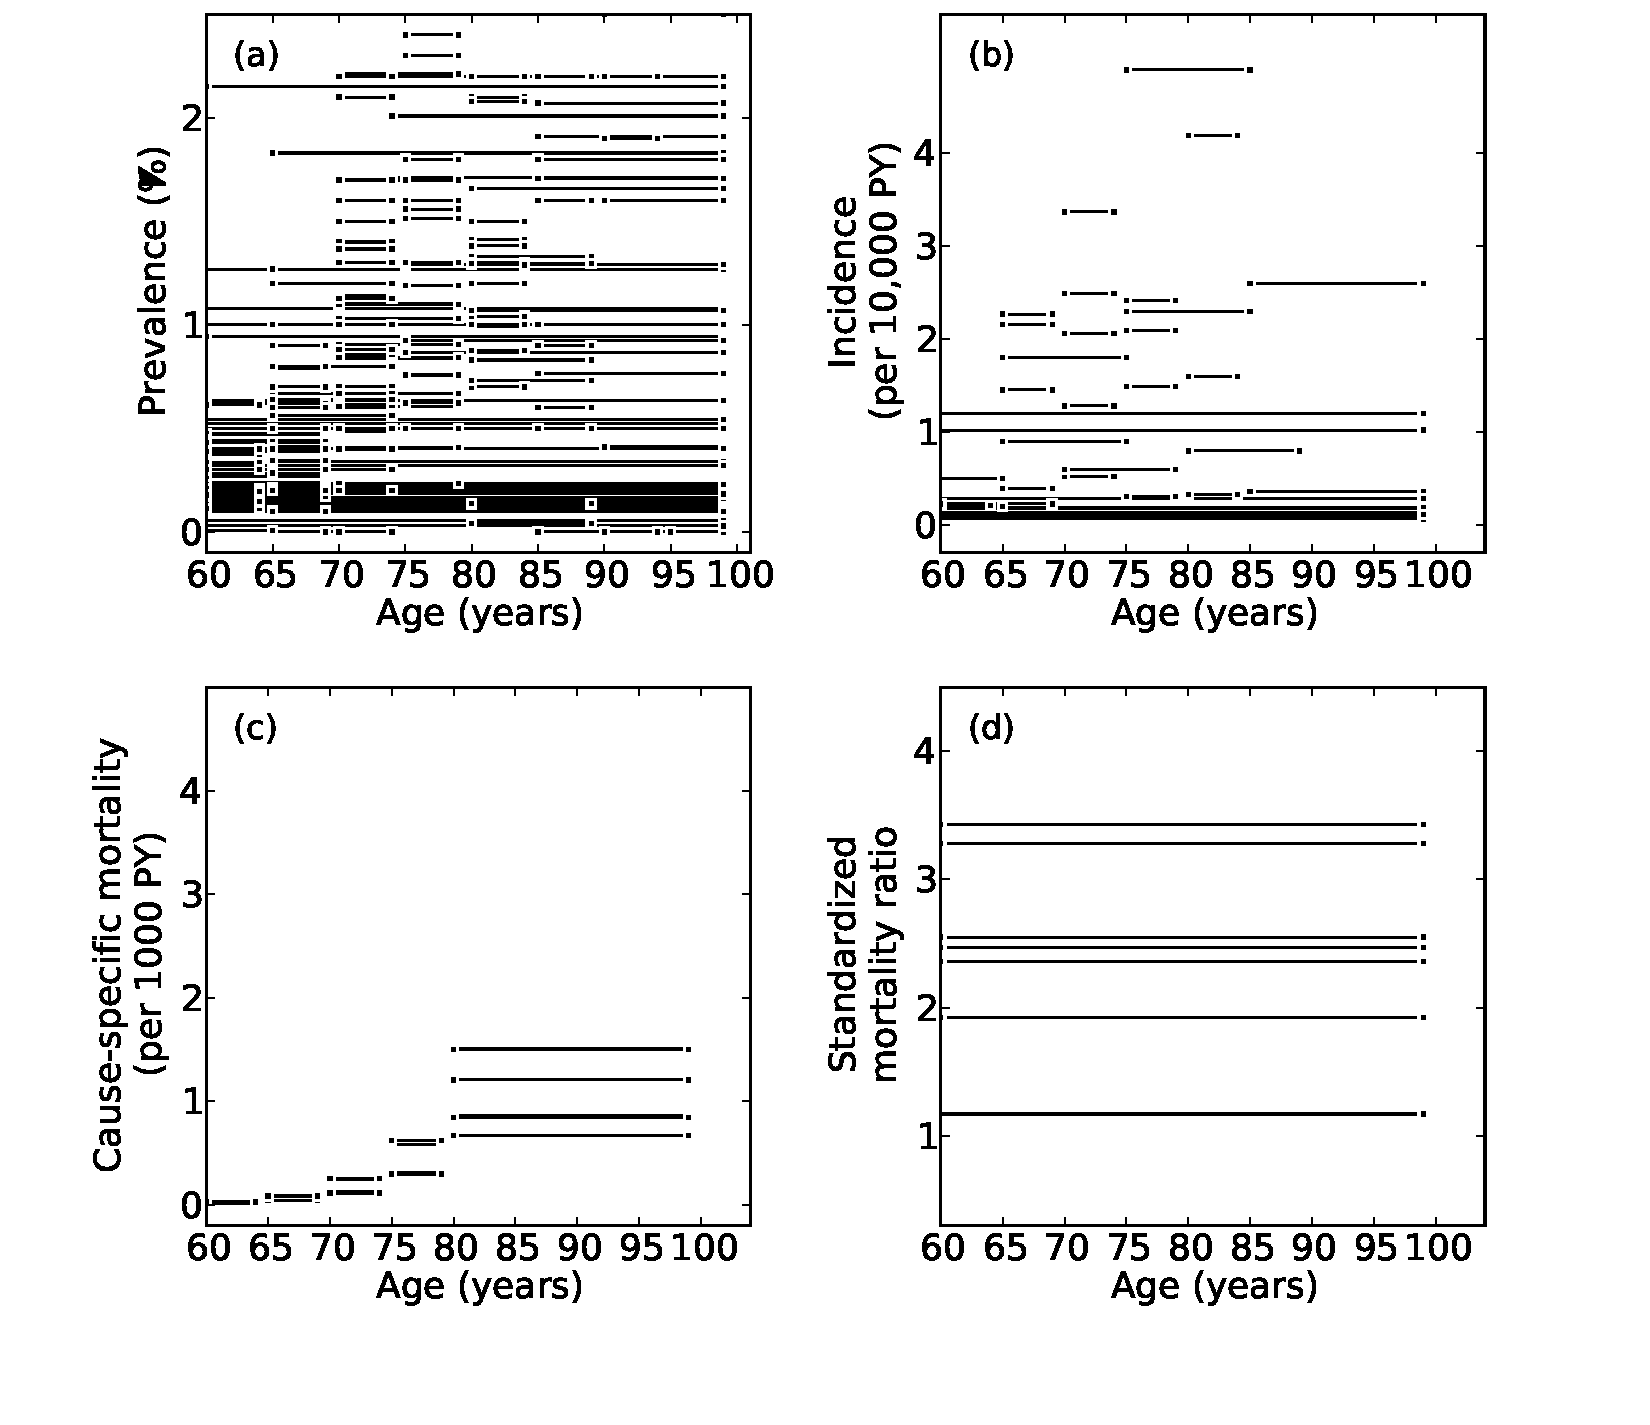
\includegraphics[width=\textwidth]{parkinsons-data.pdf}
            \caption{Data from systematic review and estimates of prevalence (panel (a)), incidence (panel (b)), cause-specific mortality (panel (c)) and the standardized mortality ratio (panel (d)) of Parkinson's disease in Western European females in 2005.}
            \label{fig:intro-parkinsons data}
        \end{center}
    \end{figure} 

Including data from 1961-2010, the data points represent the results of many different studies conducted for many different reasons.  Study level fixed effects, discussed in Chapters \ref{theory-covariate_modeling} and \ref{applications-efx_study_level}, aid the model in explaining bias resulting from differing diagnostic criteria and study populations. TK specific example.

Of the 21 regions reported in the GBD 2010 study, only 36 countries from 12 regions are represented in the systematic review.  The GBD 2010 study predicts year-age-sex estimates for all countries, even those without data.  To predict out-of-sample, country level fixed effects, as described in Chapters \ref{theory-covariate_modeling} and \ref{applications-efx_country_level}, provide a solution to this problem of missing epidemiologic data.

Nonsampling variation that cannot be explained is another problem with such noisy and heterogeneous data.  Chapters \ref{theory-covariate_modeling} and \ref{applications-rfx} explain how random effects can be used to detect systematic differences among different hierarchies of data.

It is intuitive that there is a relationship between these epidemiologic parameters: every prevalent case was once an incident case, for example.  Combining all parameters to produce internally consistent results is discussed in detail in Chapter \ref{sys-dynamics}.  Through the process of data confrontation discussed in the following chapters, the meta-analysis produces a best estimate and uncertainty bounds of disease prevalence, as shown in Figure \ref{fig:intro-parkinsons fit}.

    \begin{figure}[h]
        \begin{center}
            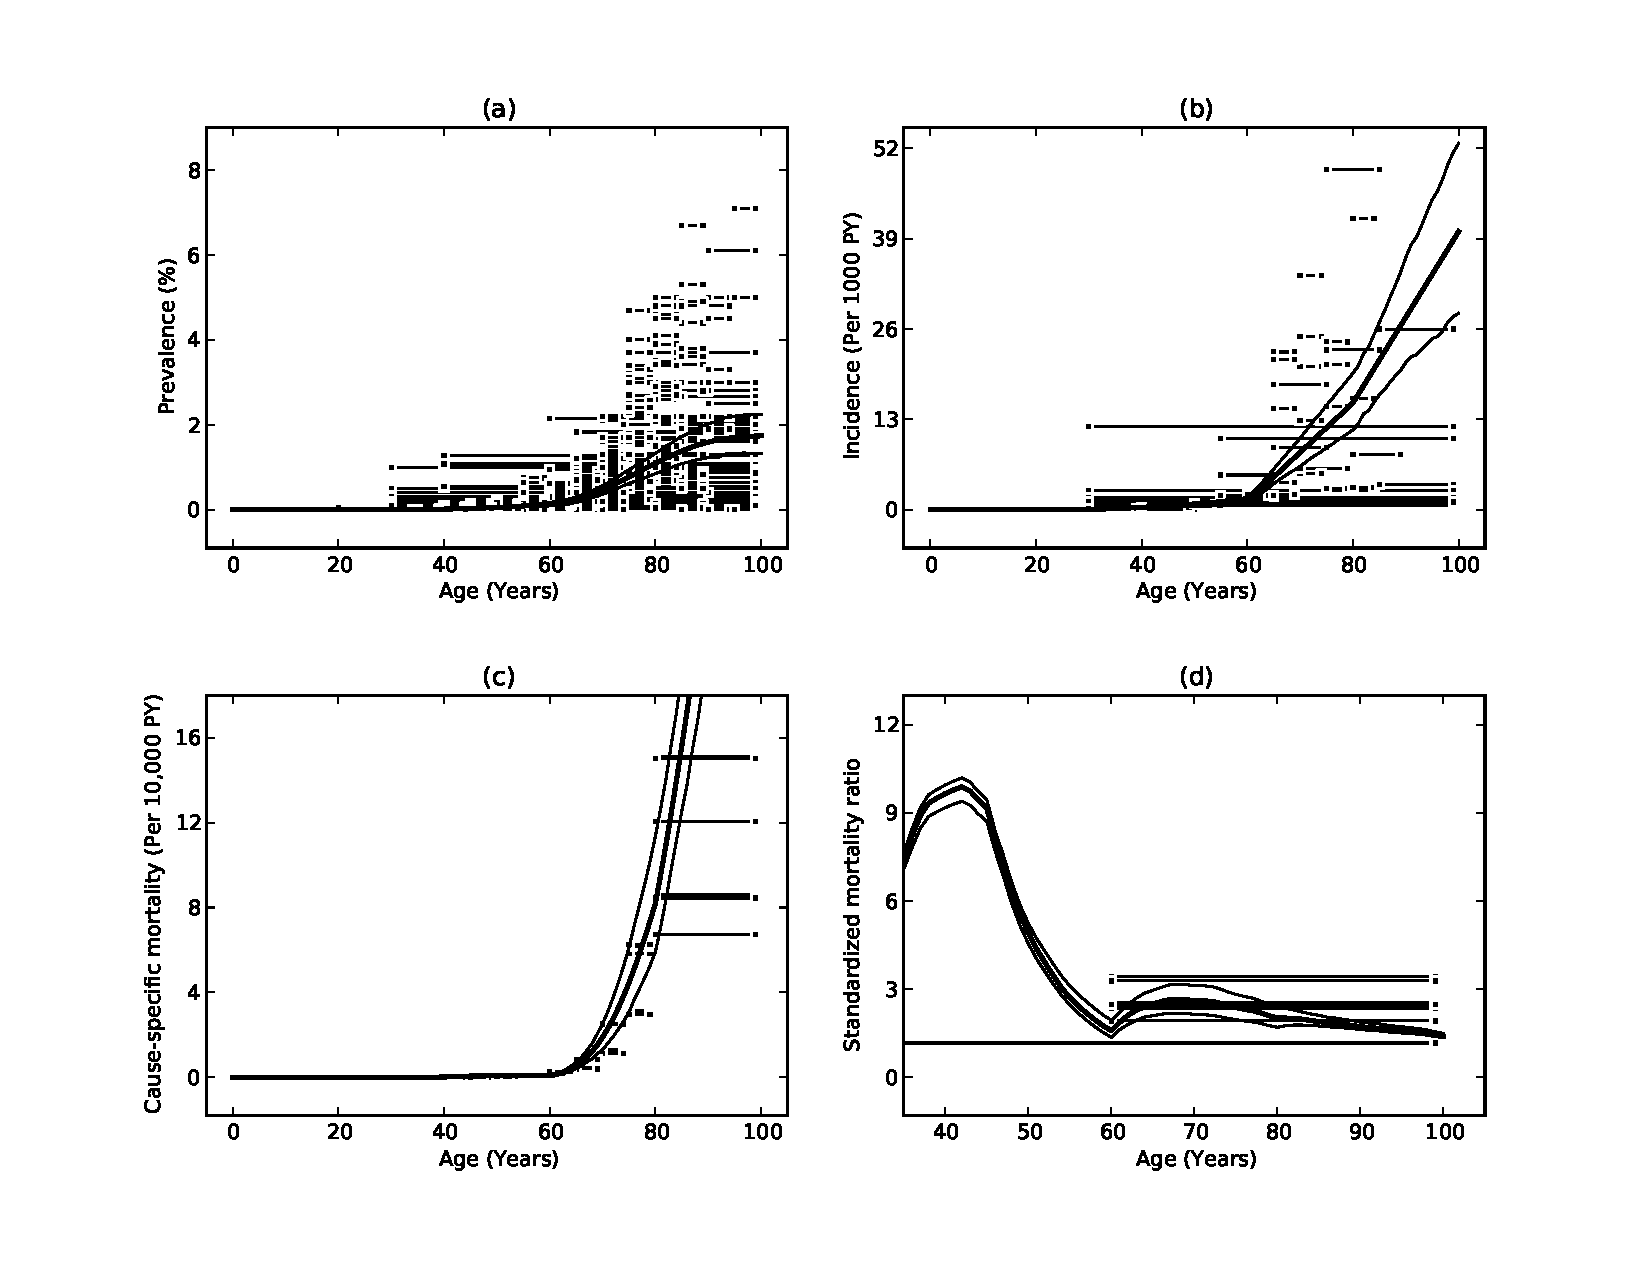
\includegraphics[width=\textwidth]{parkinsons-best.pdf}
            \caption{Data from systematic review and estimates of prevalence (panel (a)), incidence (panel (b)), cause-specific mortality (panel (c)) and the standardized mortality ratio (panel (d)) of Parkinson's disease in Western European females in 2005. TK self-contained description of contents of each panel: horizontal bar represents one row of data from systematic review.  Left and right endpoints represent age range of heterogeneous age groups, level represents level of parameter (e.g. prevalence).  Error bars are omitted, but each row of data includes a standard error or similar quantification of uncertainty as well.}
            \label{fig:intro-parkinsons fit}
        \end{center}
    \end{figure} 
